%% ==============================
\chapter{Vergleich der Methoden}
\label{ch:Vergleich}
%% ==============================

In \chapref{ch:Dimensionsreduktion} wurden grundlegende Begriffe geklärt und in
\chapref{ch:MethodenDerDimRed} fünf Methoden der Dimensionsreduktion näher betrachtet. Im jetzigen
Kapitel werden die statistischen Methoden aus \secref{ch:MethodenDerDimRed:statistisch} mit den
Machine Learning Methoden aus \secref{ch:MethodenDerDimRed:modern} empirisch auf künstlichen und
natürlichen Datensätzen verglichen. Dazu wird in \secref{ch:Vergleich:sec:Methodik} auf die
Methodik des Vergleichs eingegangen, indem die Schätzung der intrinsischen Dimension und die
eingesetzten Qualitätskriterien erläutert werden. Außerdem werden in
\secref{ch:Vergleich:sec:VerwendeteDatensaetze} die verwendeten Datensätze und in
\secref{ch:Vergleich:sec:ParameterwahlTrainingsdetails} die Parameterwahl der Methoden und
insbesondere die Architektur der Autoencoder vorgestellt. Letztlich werden in
\secref{ch:Vergleich:sec:Resultate} die Resultate des empirischen Vergleichs diskutiert.

\section{Methodik}
\label{ch:Vergleich:sec:Methodik}

Um die statistischen Methoden mit den Machine Learning Ansätzen zu vergleichen, wird die
Performance der Methoden auf mehreren künstlichen sowie natürlichen Datensätzen mit der
Vertrauenswürdigkeit, der Kontinuität und dem $\lcmc$-Kriterium gemessen. Diese Kriterien werden
jeweils für mehrere Nachbarschaftsgrößen berechnet, um eine größere Aussagekraft über die Güte der
gefundenen niedrigdimensionalen Repräsentation zu erreichen. Die Qualitätskriterien werden in
\subsecref{ch:Vergleich:sec:Methodik:subsec:Qualitaetskriterien} eingehend erläutert. Für den
Vergleich werden zwei künstliche und vier natürliche Datensätze verwendet, die in
\secref{ch:Vergleich:sec:VerwendeteDatensaetze} genauer vorgestellt werden. Insgesamt soll damit
ein Überblick über die Stärken und Schwächen der statistischen und der Machine Learning Methoden
geschafft werden. Wie bereits erwähnt, besteht zwischen Autoencodern und der
Hauptkomponentenanalyse eine enge Verbindung. Neben dem Vergleich der zwei Gruppen wird daher in
\secref{ch:Vergleich:sec:Resultate:PCA_AE} der Zusammenhang zwischen der Hauptkomponentenanalyse
und Autoencodern genauer untersucht. Der Vergleich kann mittels der im
GitHub-Repository\footnote{\url{www.github.com/MoritzM00/drcomp}} definierten Konfigurationen der
Methoden und des Trainingsskriptes repliziert werden. \rewrite{Unter Methodik könnte man auch was
	anderes verstehen. Ein bisschen mehr dazu sagen, wieso diese Vorgehensweise Sinn macht}

\subsection{Qualitätskriterien der Dimensionsreduktion}
\label{ch:Vergleich:sec:Methodik:subsec:Qualitaetskriterien}
Wie bereits in \chapref{ch:Dimensionsreduktion} erläutert, hat die Dimensionsreduktion das Ziel einer möglichst \enquote{verlustfreien} Transformation der ursprünglichen Repräsentation in eine latente Repräsentation von geringerer Dimension. Für Autoencoder bedeutet \enquote{verlustfrei} die Minimierung des Rekonstruktionsfehlers wie z.B. die quadratische Abweichung (siehe \eqref{eq:MSE_loss}). Dieser Rekonstruktionsfehler ist jedoch wie \textcite[18]{vanderMaaten.2009} hervorhebt, nicht sehr aussagekräftig für die Güte einer Dimensionsreduktion. Hinzu kommt, dass der Rekonstruktionsfehler nicht für alle Methoden berechnet werden kann, da eine inverse Transformation der niedrigdimensionalen in die ursprüngliche Repräsentation benötigt wird. Damit fällt der Rekonstruktionsfehler als geeignetes Qualitätskriterium heraus. Das immense Forschungsinteresse für Methoden der Dimensionsreduktion hat daher mit der Zeit dafür gesorgt, dass immer mehr Qualitätskriterien entwickelt wurden. \textcite{Gracia.2014} stellen einige Qualitätskriterien vor und vergleichen diese miteinander. Trotzdem gibt es in der Literatur keine eindeutige Kennzahl, die bei einem Vergleich von Dimensionsreduktionsmethoden standardmäßig eingesetzt wird \parencite[vgl.][1 -- 2]{Lee.2009}. Stattdessen bedient man sich mehrerer Kennzahlen, die
unterschiedliche Dinge bestrafen und versucht so die Stärken und Schwächen einer
Dimensionsreduktionsmethode zu erkennen \parencite[486]{Venna.2001}. Die im Folgenden vorgestellten Qualitätskriterien versuchen die Güte
mithilfe von Rängen zu quantifizieren.

Im ausführlichen Benchmark von \textcite{vanderMaaten.2009} wird auf den Generalisierungsfehler
eines 1-Nächste-Nachbar Klassifikators, sowie auf die zwei Kennzahlen
\newterm{Vertrauenswürdigkeit} (engl. \textit{Trustworthiness}) und \newterm{Kontinuität} (engl.
\textit{Continuity}) \parencites{Venna.2001}{Venna.2006} gesetzt. Die Vertrauenswürdigkeit und die Kontinuität sind
rang-basierte Qualitätskriterien und werden auch in diesem Vergleich eingesetzt. Daneben gibt es
noch viele weitere rangbasierte Qualitätskriterien, welche einheitlich durch die sogenannte
\newterm{Co-Ranking Matrix} \parencite[1432]{Lee.2009} ausgedrückt werden können. Ebenso können die Vertrauenswürdigkeit und
Kontinuität über die Co-Ranking Matrix berechnet werden \parencite[1433]{Lee.2009}. Für eine ausführliche Behandlung dessen wird auf \textcite{Lee.2009}
verwiesen. In dieser Arbeit werden drei Kriterien verwendet: (1) Die Vertrauenswürdigkeit und (2)
die Kontinuität einer Dimensionsreduktion, sowie (3) das \newterm{Local Continuity Meta-Criterion}
(LCMC). Diese werden im Folgenden genauer betrachtet. \nomenclature[Z]{LCMC}{Local Continuity
	Meta-Criterion}
\subsubsection{Vertrauenswürdigkeit und Kontinuität}
\label{ch:Vergleich:sec:Methodik:subsec:Qualitaetskriterien:TC}
Diese beiden Kennzahlen basieren auf der Idee des Erhalts von Nachbarschaften (engl.
\textit{neighborhood preservation}) einer Dimensionsreduktion. Sie bilden also ab, wie gut die
lokale Struktur erhalten wird. Eine $K$-Nachbarschaft $\set{M}_i(K)$ eines Punktes $\vect{x}_i$ ist
definiert als die Menge der Indizes der $K$-nächsten Punkte zu $\vect{x}_i$ ($i = 1, \ldots, n$).
Analog kann die $K$-Nachbarschaft $\widetilde{\set{M}}_i(K)$ des dazugehörigen niedrigdimensionalen
Punktes $\vect{y}_i$ definiert werden. Diese Nachbarschaft wird in einer Dimensionsreduktion
erhalten, wenn $\set{M}_i(K) = \widetilde{\set{M}}_i(K)$, das heißt die Nachbarschaften bleiben von
der Dimensionsreduktion unverändert.

Zum einen kann es nun passieren, dass Punkte, die \textit{vor} der Projektion weit weg voneinander
lagen, \textit{nach} der Projektion aber nah beieinander sind. Mit anderen Worten können Punkte,
die eigentlich unterschiedlich sind, nun ähnlich erscheinen. Aus diesem Grund sagt man, dass die
Vertrauenswürdigkeit der Dimensionsreduktion niedrig ist. Zum anderen ist der gegenteilige Fall
möglich. Nah beieinander liegende Punkte sind nach der Projektion weit weg voneinander. Dies
reduziert die Kontinuität einer Dimensionsreduktion \parencite[486 -- 487]{Venna.2001}.

Formal definiert man zusätzlich zu den Nachbarschaftsmengen von oben die beiden Mengen
$\set{U}_i(K)$ und $\set{V}_i(K)$ wie folgt:
\begin{gather}
	\set{U}_i(K) =  \left\{ j \in \N \mid j \notin \set{M}_i(K) \land j \in \widetilde{\set{M}}_i(K) \right\} \, , \\
	\set{V}_i(K) =  \left\{ j \in \N \mid j \in \set{M}_i(K) \land j \notin \widetilde{\set{M}}_i(K) \right\} \, .
\end{gather}
Diese beiden Mengen bilden lediglich die zwei intuitiv besprochenen Fälle im vorherigen Absatz mathematisch ab. Hierbei entspricht $\set{U}_i(K)$ dem ersten und $\set{V}_i(K)$ dem zweiten Fall.
Damit kann die Vertrauenswürdigkeit $T(K)$ als
\begin{equation}
	T(K) = 1 - \frac{2}{nK(2n - 3K - 1)} \sum_{i = 1}^{n}\sum_{j \in \set{U}_i(K) } \left( r­_{\vect{y}}(i, j) - K \right)
\end{equation}
definiert werden \parencite[487]{Venna.2001}, wobei $r_{\vect{y}}(i, j)$ den Rang von des niedrigdimensionalen Vektors
$\vect{y}_j$ bezeichnet, wenn die Datenpunkte absteigend nach der euklidischen Distanz von
$\vect{y}_i$ geordnet sind. Der Term vor der Summation skaliert das Qualitätskriterium so, dass $0
	\leq T(K) \leq 1$ gilt.\footnote{Dies gilt nur für den Fall, dass $K < n/2$ gilt.} Ein Wert von
$T(K) = 1­$ spricht für eine hohe Vertrauenswürdigkeit.

Analog wird die Kontinuität $C(K)$ über $\set{V}_i(K)$ wie folgt definiert
\begin{equation}
	C(K) = 1 - \frac{2}{nK(2n - 3K - 1)} \sum_{i = 1}^{n}\sum_{j \in \set{V}_i(K) } \left( r_{\vect{x}}(i, j) - K \right) \, ,
\end{equation}
wobei $r_{\vect{x}}(i, j)$ nun den Rang zwischen den Datenpunkten in der hochdimensionalen Repräsentation bezeichnet \parencite[487]{Venna.2001}. Auch hier gilt $0 \leq C(K) \leq 1$ und höher ist besser. Die Kontinuität
misst also, wie gut die ursprünglichen Nachbarschaften erhalten werden.

Üblicherweise werden die beiden Kriterien für mehrere Werte der Nachbarschaftsgröße $K$ berechnet und in einer Abbildung dargestellt. So entfällt die etwas willkürliche Wahl einer spezifischen Nachbarschaftsgröße und ermöglicht die Betrachtung von sowohl kleinen als auch größeren Nachbarschaften.
% \subsubsection{Die Co-Ranking Matrix}
% Ein Eintrag $q_{kl}$ der Co-Ranking Matrix $\mat{Q}$ ist die Anzahl der Paare von Datenpunkten $(i,
% 	j)$, die den Rang $r_{\vect{x}}(i, j) = k$ in der hochdimensionalen und den Rang $r_{\vect{y}}(i,
% 	j) = l$ in der niedrigdimensionalen Repräsentation haben.

\subsubsection{Local Continuity Meta-Criterion}
\label{ch:Vergleich:sec:Methodik:subsec:Qualitaetskriterien:LCMC}
Das Local Continuity Meta-Criterion (LCMC), entwickelt von \textcite{Chen.2009}, ist ebenso wie die Vertrauenswürdigkeit und Kontinuität ein rang-basiertes Qualitätskriterium. LCMC betrachtet die Überschneidung der $K$-Nachbarschaften in der ursprünglichen und latenten Repräsentation. Nimmt man wieder die $K$-Nachbarschaften aös $M_i(K)$ und $\widetilde{M}_i(K)$ an, das heißt die Indexmengen der $K$-Nachbarschaften in der ursprünglichen beziehungsweise latenten Repräsentation, dann lässt sich das LCMC wie folgt berechnen \parencite[212]{Chen.2009}:
\begin{equation}
	\label{eq:LCMC}
	\text{LCMC}(K) = \frac{1}{nK} \sum_{i=1}^{n} \left( \left| \set{M}_i(K) \cap \widetilde{\set{M}}_i(K) \right| \right) - \frac{K}{n - 1} \,,
\end{equation}
wobei $­|\cdot|$ die Kardinalität einer Menge und $\set{A} \cap \set{B}$ den Durchschnitt zweier Mengen $\set{A}$ und $\set{B}$ bezeichnet. Der Term vor der Summation skaliert auch dieses Kriterium auf den Wertebereich zwischen Null und Eins, wobei LCMC$(K) = 1$ den besten Wert darstellt. Die durschnittliche Überschneidung der beiden Indexmengen wird wie in \eqref{eq:LCMC} ersichtlich noch um einen additiven Term korrigiert. Dieser Term entspricht dem Erwartungswert einer zufälligen Überschneidung und kann durch eine hypergeometrische Verteilung mit $K$ Defekten aus $n - 1$ modelliert werden \parencite[213]{Chen.2009}. Diese sogenannte Basislinie (engl. \textit{Baseline}) wird mit steigendem
$K$ größer, so dass das Kriterium für den maximalen Wert der Nachbarschftsgröße $K = n - 1$ den
Wert Null annimmt. Aus diesem Grund besitzt das LCMC ein wohldefiniertes Maximum. Allerdings sind
kleinere Werte von $K$ oftmals wichtiger, um beispielsweise die Erhaltung der Struktur einer
Mannigfaltigkeit zu messen.

\subsection{Schätzen der intrinsischen Dimension}
\label{ch:Vergleich:sec:Methodik:subsec:SchaetzenDerIntrinsischenDim}

Bis jetzt wurde immer angenommen, dass die intrinsische Dimension $d$ der Daten bekannt ist, da die
meisten Dimensionsreduktionsmethoden die intrinsische Dimension nicht selbst berechnen. Das
Schätzen der intrinsischen Dimension ist also ein nicht unwichtiges Teilproblem der
Dimensionsreduktion, da eine Unterschätzung von $d$ dazu führt, dass relevante Strukturen
zwangsweise verloren gehen \parencite[1]{Levina.2004}. Erschwert wird dieses Problem durch die Tatsache, dass es viele
Definitionen der intrinsischen Dimension und damit auch viele unterschiedliche Schätzer gibt. Im
Folgenden soll ein kurzer Überblick verschafft werden, jedoch geht eine detaillierte Behandlung der
Schätzung über den Rahmen dieser Arbeit hinaus. Daher wird für einen Überblick und Vergleich dieser
Schätzer auf \textcites{Campadelli.2015}{Bac.2021}{Verveer.1995} verwiesen.

In \secref{ch:Dimensionsreduktion:MannigfaltigkeitenIntrinsDim} haben wir die \textit{topologische
	Dimension} kennengelernt, welche sich in der Literatur zur Strukturerkennung durchgesetzt hat \parencite[1]{Campadelli.2015}. Allerdings bringt diese Definition praktische Schwierigkeiten mit sich,
weswegen die meisten Schätzer der intrinsischen Dimension auf der damit verwandten
\textit{fraktalen Dimension} wie zum Beispiel der Schätzer der Korrelationsdimension \parencite{Camastra.2002} basieren. Daneben gibt es noch Nächste-Nachbar-basierte Schätzer \parencite[1]{Campadelli.2015}. Zu dieser Kategorie gehört auch der weitverbreitete und in dieser
Arbeit verwendete \newterm{Maximum Likelihood Schätzer} von \textcite{Levina.2004}. Diese Schätzer
betrachten die Verteilung der Nachbarschaft eines Punktes $\rvect{x}$ als Funktion der
intrinsischen Dimension -- üblicherweise innerhalb einer kleinen Kugel um $\rvect{x}$
\parencite[8]{Campadelli.2015}. Der Maximum Likelihood Schätzer nimmt an, dass die Beobachtungen, die
in einer solchen Kugel liegen, einem homogenen Poisson-(Zähl-)Prozess\unsure{Hier in der Fußnote
	etwas dazu erzählen} folgen
\parencite[2]{Levina.2004}. Dieser Prozess hängt von $d$ ab, weshalb mittels der Maximum Likelihood
Methode ein Schätzwert $\estNormal{d}$ für einen fixen Punkt $\rvect{x}_i$ als
\begin{equation}
	\estNormal{d}_K(\vect{x}_i) = \left( \frac{1}{K - 1} \sum_{j=1}^{K - 1} \log \frac{T_K(\vect{x}_i)}{T_j(\vect{x}_i)} \right)^{-1}
\end{equation}
berechnet werden kann \parencite[4]{Levina.2004}. Hierbei ist $K$ die Anzahl der nächste Nachbarn und $T_{K}(\vect{x}_i)$ die
euklidische Distanz von $\vect{x}_i$ zu seinem $K$-ten Nachbar. Dies ist jedoch nur eine lokale
Schätzung für einen fixen Punkt $\vect{x}_i$. Um eine globale Schätzung zu erhalten, wird der
Mittelwert über alle Beobachtungen $\vect{x}_i$ mit $i = 1, \ldots, n$ gebildet.
\section{Verwendete Datensätze}
\label{ch:Vergleich:sec:VerwendeteDatensaetze}
Es werden sowohl künstliche als auch natürliche Datensätze eingesetzt, um Eigenschaften der
verschiedenen Methoden miteinander zu vergleichen. Eine Übersicht über die Dimensionen und Stichprobengrößen der verwendeten Datensätze befindet sich in Tabelle \ref{tab:uebersicht-datensaetze}.

\subsection{Künstliche Datensätze}
\label{ch:Vergleich:sec:VerwendeteDatensaetze:kuenstlich}
Zu den künstlichen Datensätzen gehört die weitverbreitete \textit{Swiss Roll} und der \textit{Twin Peaks} Datensatz,
\begin{figure}[ht]
	\begin{center}
		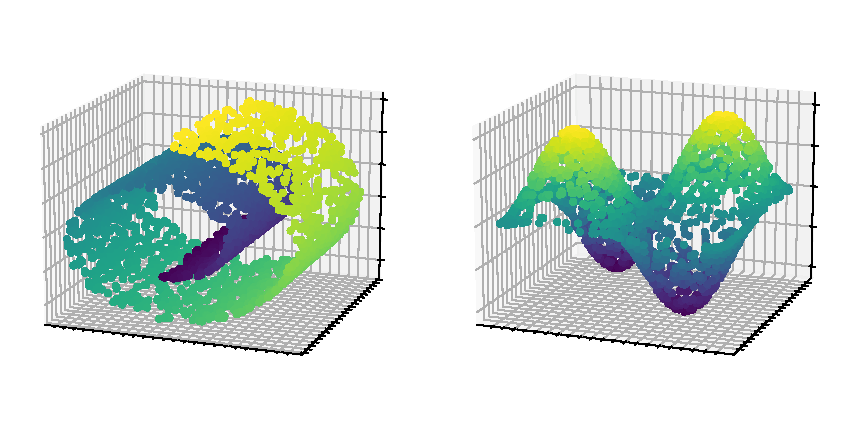
\includegraphics{artificial_datasets.pdf}
	\end{center}
	\caption[Künstliche Datensätze]{\figleft Die Swiss Roll. Die intrinsische Dimension beträgt zwei, weil die Daten auf einer \enquote{eingerollten Ebene} liegen. Die Dimensionsreduktionsmethoden müssen die Swiss Roll \enquote{entfalten}, um eine zweidimensionale Repräsentation zu erhalten. \figright Der Twin Peaks Datensatz. Dieser besteht aus je zwei spitzen Bergen, die nach oben und unten zeigen. Auch dieser Datensatz hat eine intrinsische Dimension von zwei. Intuitiv gesehen kann man sich lokal nur nach rechts oder links bewegen, d.h. die Twin Peaks homöomorph zum $\real^2$ sind.}
	\label{fig:ArtificialDatasets}
\end{figure}
die in \figref{fig:ArtificialDatasets} dargestellt sind.
Beide künstlichen Datensätze bestehen aus 5 000 Datenpunkten und haben eine extrinsische Dimension von drei und eine intrinsische
Dimension von zwei. Dies erlaubt eine visuelle Betrachtung der Datensätze und der gefundenen
latenten Räume, schränkt aber gleichzeitig die Architektur eines (unterbestimmten) Autoencoders
ein. Künstliche Datensätze sind aber nicht zwangsweise aussagekräftig für die Performance auf echten Datensätzen, weswegen zusätzlich fünf natürliche Datensätze hinzugezogen werden.

\subsection{Natürliche Datensätze}
\label{ch:Vergleich:sec:VerwendeteDatensaetze:natuerlich}
Natürliche
Datensätze weisen laut empirischen Ergebnissen \addref oft komplexe nichtlineare Zusammenhänge
auf und sind daher für die Dimensionsreduktion anspruchsvoller als kleine, künstlich generierte
Datensätze. Der Nachteil besteht darin, dass die intrinsische Dimension in der Regel deutlich über
zwei liegt und daher der latente Raum nicht visualisiert werden kann. Nichtsdestotrotz liefern die
Qualitätskriterien hinreichende gute Indizien für die Performance der Methoden. Bei den natürlichen
Datensätzen wurden größtenteils Bilddatensätze, aber auch ein Datensatz mit Genausprägungen ausgewählt, da diese eine
hohe extrinsische Dimension aufweisen und daher für die Dimensionsreduktion gut geeignet sind.
Konkret wurde (1) der \textit{MNIST}-Datensatz \parencite{LeCun.2010}, (2) der \textit{Olivetti Faces}-Datensatz
\footnote{\url{https://cam-orl.co.uk/facedatabase.html}}, (3) der \textit{Fashion MNIST}-Datensatz \parencite{Xiao.8252017}, (4) der \textit{Facial Emotion Recognition} (FER) Datensatz \parencite{DumitruIanGoodfellowWillCukierskiYoshuaBengio.2013} und (5) der
\textit{ICMR}-Datensatz\footnote{\url{https://www.kaggle.com/datasets/shibumohapatra/icmr-data?select=labels.csv}}
ausgewählt, um die Performance der Dimensionsreduktionsmethoden auf natürlichen Datensätzen zu
evaluieren. Der weitverbreitete MNIST-Datensatz besteht aus 60 000 Grauton-Bildern von
handgeschriebenen Zahlen in der Auflösung $28 \times 28$. Die Anzahl der Pixel und damit die
extrinsische Dimension beträgt 784. Der \textit{Olivetti Faces}-Datensatz enthält Bilder von
Gesichtern aus zehn unterschiedlichen Positionen von 40 Personen und ist damit der kleinste
natürliche Datensatz in diesem Vergleich mit 400 Bildern. Die Bilder haben eine Auflösung von $64
	\times 64$, was einer extrinsischen Dimension von 4096 entspricht. Der Fashion MNIST-Datensatz
besteht aus 60 000 Bildern von zehn unterschiedlichen Kleidungsstücken. Die extrinsische Dimension
ist ebenso wie bei MNIST 784. FER-Datensatz besteht aus 28 709 Bildern von Gesichtern mit sieben
unterschiedlichen Emotionen. Die Bilder haben eine Auflösung von $48 \times 48$ und sind damit
2304-dimensional. Beispiele der Bild-Datensätze sind in \figref{fig:Dataset_samples} zu finden.
\begin{figure}
	\begin{center}
		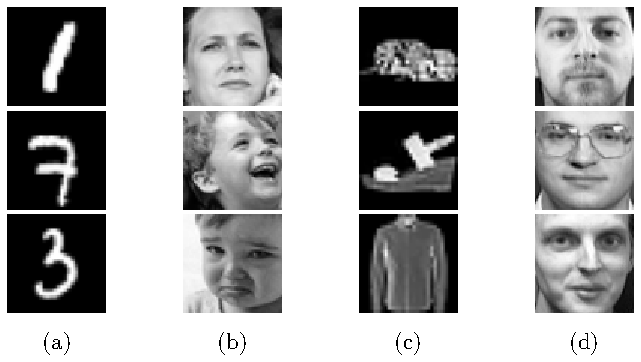
\includegraphics{dataset_samples.pdf}
	\end{center}
	\caption[Beispielbilder der natürlichen Datensätze]{Zu sehen sind je vier Beispielbilder der natürlichen Bilddatensätze aus dem Vergleich: \captiona Handgeschriebene Zahlen aus dem MNIST-Datensatz \captionb Gesichter mit unterschiedlichen Emotionen aus dem FER-Datensatz \captionc Verschiedene Kleidungsstücke aus dem Fashion MNIST-Datensatz \captiond Bilder der Gesichter unterschiedlicher Personen aus zehn Blickwinkeln (Olivetti Faces-Datensatz)}
	\label{fig:Dataset_samples}
\end{figure}

\nomenclature[Z]{MNIST}{Modified National Institute of Standards and Technology (Datensatz)}
\nomenclature[Z]{FER}{Facial Emotion Recognition (Datensatz)}
\nomenclature[Z]{ICMR}{Indian Council of Medical Research (Datensatz)}

Letztlich enthält der ICMR-Datensatz Genausprägungen von 801 Personen, die mit fünf
unterschiedlichen Arten von Krebs diagnostiziert wurden. Der Datensatz enthält Genausprägungen von
über 20 000 Genen, womit dieser Datensatz die höchste extrinsische Dimension im Vergleich besitzt.
In Tabelle \ref{tab:uebersicht-datensaetze} sind die extrinsischen und intrinsischen Dimensionen,
sowie die Stichprobengrößen der Datensätze zusammengefasst. Die intrinsischen Dimensionen sind die
Schätzungen des in \subsecref{ch:Vergleich:sec:Methodik:subsec:SchaetzenDerIntrinsischenDim}
erläuterten Maximum Likelihood Schätzers für den jeweiligen Datensatz.

\begin{table}[]
	\centering
	\ra{1.2}
	\begin{tabular}{@{}lrrr@{}}
		\toprule
		Datensatz      & extrinsische Dimension $D$ & intrinsische Dimension $d$ & Stichprobengröße $n$ \\ \midrule
		Swiss Roll     & 3                          & 2                          & 5 000                \\
		Twin Peaks     & 3                          & 2                          & 5 000                \\
		MNIST          & 784                        & 15                         & 60 000               \\
		Fasion MNIST   & 784                        & 18                         & 60 000               \\
		Olivetti Faces & 4 096                      & 9                          & 400                  \\
		FER            & 2 304                      & 26                         & 28 709               \\
		ICMR           & 20 531                     & 22                         & 801                  \\
		\bottomrule
	\end{tabular}
	\caption[Übersicht über die extrinsischen und intrinsischen Dimensionen, sowie die Stichprobengröße der in diesem Vergleich verwendeten Datensätze]{Übersicht über die extrinsischen und intrinsischen Dimensionen, sowie die Stichprobengröße der in diesem Vergleich verwendeten Datensätze. Bei Bilddatensätzen entspricht die extrinsische Dimension der Anzahl der Pixel im Bild. Die intrinsische Dimension wurde mit dem Maximum Likelihood Schätzer aus \subsecref{ch:Vergleich:sec:Methodik:subsec:SchaetzenDerIntrinsischenDim} mit einer Nachbarschaftsgröße $K=5$ geschätzt.}
	\label{tab:uebersicht-datensaetze}
\end{table}

\section{Trainingsdetails und Parameterwahl}
\label{ch:Vergleich:sec:ParameterwahlTrainingsdetails}

In diesem Abschnitt werden die gewählten (Hyper-)Parameter und Details des Trainierens der
Dimensionsreduktionsmethoden vorgestellt. Eine Übersicht ist in
Tabelle~\ref{tab:uebersicht-parameter} zu finden. Alle Datensätze wurde vor dem Anwenden der
Dimensionsreduktionsmethoden standardisiert, das heißt $\mat{X}$ weist einen spaltenweisen
Erwartungswert von Null und eine spaltenweise Varianz von Eins auf. Für die Evaluierung der
Methoden wurde aufgrund von Restriktionen der Rechenleistung (insbesondere des Arbeitsspeichers)
ein Downsampling auf maximal 15 000 Stichproben durchgeführt.\footnote{Die Evaluierung ist aufgrund
	der Berechnung der Co-Ranking-Matrix speicherintensiv, da diese maximal $(n-1) \times (n-1)$ groß
	ist und damit quadratisch mit $n$ ansteigt. Um die Qualitätskriterien für den MNIST-Datensatz zu
	berechnen, werden für $n=25 000$ circa 25 GB Arbeitsspeicher benötigt.} Dies ist allerdings nur für
den MNIST- und FER-Datensatz von Relevanz. Alle anderen Datensätze haben weniger Stichproben.

Für die Hauptkomponentenanalyse gibt es neben der Anzahl der zu behaltenden Hauptkomponenten keine
Parameter. Die Anzahl der Hauptkomponenten entspricht der intrinsischen Dimension, welche vom
Datensatz abhängt und für alle Methoden identisch ist. Dies trifft analog auf Kernel PCA und auf
Locally Linear Embedding zu. Für Autoencoder bestimmt die intrinsische Dimension die Größe der
Bottleneck-Schicht. Für Kernel PCA wird ein Gaußscher Kernel eingesetzt, wofür ein Hyperparameter
$\sigma$ gewählt werden kann. Die Werte $\sigma \in \{ 0.1, 0.25, 0.75, 1, 2, 5\}$ wurden getestet
und der beste Durchlauf ausgewählt. Für ICMR und Olivetti Faces lieferten diese Werte sehr
schlechte Ergebnisse, weswegen auf diesen Datensätzen zusätzlich die Werte $\{ 0.001, 0.0001,
	0.00001\}$ getestet wurden. Für Locally Linear Embedding gibt es zwei Parameter: (1) einen
Parameter $K$, der die Größe der verwendeten Nachbarschaft kontrolliert und (2) eine
Regularisierungs-Konstante $\epsilon$, die auf die Diagonale der lokalen Kovarianzmatrix addiert
wird.

Den statistischen Methoden gegenüber haben Autoencoder deutlich mehr Freiheitsgrade, um die
Architektur zu bestimmen. Die wichtigsten Parameter sind die Anzahl der Schichten $m$, sowie die
Anzahl an Neuronen pro Schicht und die Wahl der Aktivierungsfunktionen. Daneben gibt es noch viele
weitere Freiheitsgrade für das Trainieren des Autoencoders, welche teilweise vom Datensatz
abhängen. Diese wurden für alle Autoencoder nahezu identisch gewählt und werden in
Appendix~\ref{ch:Appendix:Architektur-Details} genauer erläutert. Für beide künstlichen Datensätze
und für den Olivetti Faces-Datensatz wird ein dreischichtiger\rewrite{das stimmt nicht mehr}
Autoencoder eingesetzt. Für alle anderen Datensätze wird ein fünfschichtiger Autoencoder trainiert.
Alle vollvernetzten Autoencoder und der Contractive Autoencoder verwenden
Sigmoid-Aktivierungsfunktionen im Encoder und Decoder. Auf Bilddatensätzen wurden zusätzlich
Convolutional Autoencoder trainiert, deren Architekturen an \textcite[14]{Ghosh.2019} angelehnt und
ebenfalls in Appendix~\ref{ch:Appendix:Architektur-Details} spezifiziert sind.

\begin{table}[ht]
	\tymax=300pt
	\centering
	\ra{1.3}
	\begin{tabulary}{\linewidth}{CC}
		\toprule
		Methode                            & Parameter                                                            \\ \midrule
		Hauptkomponentenanalyse (PCA)      & --                                                                   \\
		Kernel PCA                         & $\kappa(\vect{x}_1, \vect{x}_2) = \exp(- \norm{\vect{x}_1 - \vect{x}_2}^2/(2\sigma))$, $\sigma=\sfrac{1}{D}$ \\
		Locally Linear Embedding (LLE)     & $K=10$, $\epsilon=1\mathrm{e}{-3}$                                   \\
		Autoencoder (AE)                   & $m \in \{3, 5\}$, Sigmoid-Aktivierungsfunktion \newline (siehe
		Appendix~\ref{ch:Appendix:Architektur-Details})                                                           \\  Contractive Autoencoder (CAE) & $m = 3$, $\lambda=1\mathrm{e}{-4}$,
		Sigmoid-Aktivierungsfunktion (siehe Appendix~\ref{ch:Appendix:Architektur-Details})                       \\
		Convolutional Autoencoder (ConvAE) & $m > 5$, ReLU-Aktivierungsfunktion \newline (siehe
		Appendix~\ref{ch:Appendix:Architektur-Details})                                                           \\ \bottomrule
	\end{tabulary}
	\caption[Übersicht über die verwendeten Parameter der Methoden]{Übersicht über die verwendeten Parameter. Hierbei ist $\kappa$ die Kernel-Funktion, $D$ die extrinsische Dimension des Datensatzes, $K$ die Nachbarschaftsgröße, $\epsilon$ eine Regularisierungskonstante für LLE, $m$ die Anzahl der Schichten im Autoencoder und $\lambda$ eine multiplikative Konstante für den kontrahierenden Fehlerterm des CAE.}
	\label{tab:uebersicht-parameter}
\end{table}
\section{Resultate}
\label{ch:Vergleich:sec:Resultate}

In diesem Abschnitt werden die Resultate des empirischen Vergleichs vorgestellt. Dazu werden die
Werte der verschiedenen Qualitätskriterien auf den künstlichen und natürlichen Datensätzen in
Abhängigkeit der Nachbarschaftsgröße $K$ abgebildet. Die verschiedenen Methoden wurden mit den im
vorhergehenden \secref{ch:Vergleich:sec:ParameterwahlTrainingsdetails} erläuterten Parametern auf
den künstlichen und natürlichen Datensätzen trainiert und hinsichtlich der in
\secref{ch:Vergleich:sec:Methodik:subsec:Qualitaetskriterien} vorgestellten Qualitätskriterien für
eine Nachbarschaftsgröße von $1 \leq K \leq 100$ evaluiert. Einige der Abbildungen für die
Qualitätskriterien sind im Appendix \ref{ch:Appendix:Qualitaetskriterien} zu finden. In
\secref{ch:Vergleich:sec:Resultate:kuenstlich} werden die Ergebnisse auf den künstlichen
Datensätzen und in \secref{ch:Vergleich:sec:Resultate:natuerlich} die Ergebnisse auf den
natürlichen Datensätzen diskutiert. Letztlich wird in \secref{ch:Vergleich:sec:Resultate:PCA_AE}
der Zusammenhang zwischen der Hauptkomponentenanalyse und Autoencodern empirisch untersucht.

\subsection{Resultate auf künstlichen Datensätzen}
\label{ch:Vergleich:sec:Resultate:kuenstlich}

Die Qualitätskriterien für den Swiss Roll Datensatz sind in \figref{fig:SwissRollMetrics}
\begin{figure}[ht]
	\begin{center}
		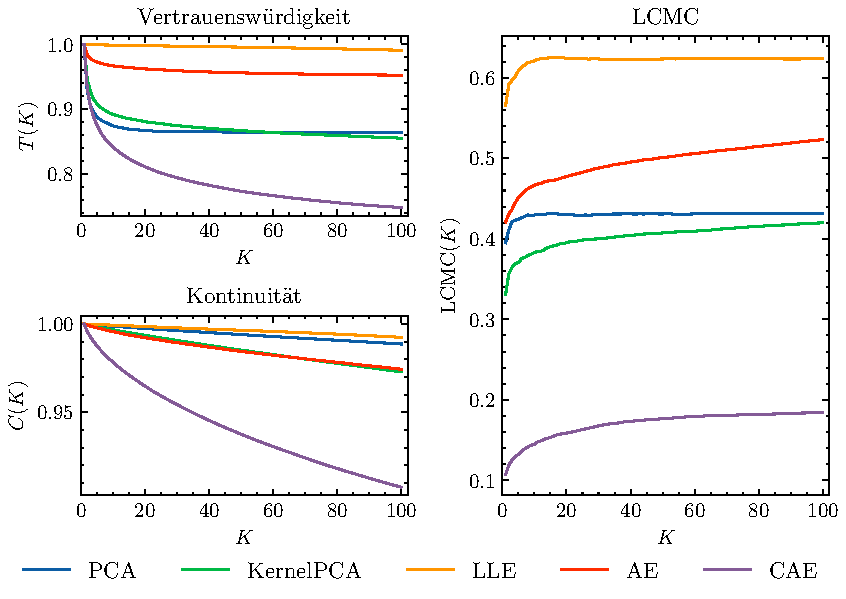
\includegraphics{SwissRoll_comparison.pdf}
	\end{center}
	\caption[Qualitätskriterien für die Swiss Roll]{Die Vertrauenswürdigkeit und Kontinuität der Dimensionsreduktion, sowie das Local Continuity Meta-Criterion (LCMC) für den Swiss Roll Datensatz. Locally Linear Embedding (LLE) schneidet mit Abstand am besten ab. Die restlichen Methoden unterscheiden sich nicht stark, lediglich bei der Vertrauenswürdigkeit können sich die Kernel PCA und der Contractive Autoencoder etwas nach oben absetzen. Die PCA und der Autoencoder sind hinsichtlich der Kontinuität und des LCMC ähnlich. (Eigene Darstellung)}
	\label{fig:SwissRollMetrics}
\end{figure}
und die Qualitätskriterien für den Twin Peaks Datensatz in \figref{fig:TwinPeaksMetrics} abgebildet. Wie dort zu erkennen ist, zeigt Locally Linear Embedding eine starke Performance auf den beiden künstlichen Datensätzen. Der Autoencoder kann sich hinsichtlich des Twin Peaks Datensatzes von den restlichen Methoden abheben. Bei der Swiss Roll ist dies jedoch nicht der Fall. Hier sind die PCA, die Kernel PCA, sowie beide Varianten des Autoencoders relativ ähnlich.

Wie eingangs in \subsecref{ch:Vergleich:sec:VerwendeteDatensaetze:kuenstlich} erwähnt, ist die
Möglichkeit der Visualisierung der latenten Repräsentation ein Vorteil der Evaluierung auf
künstlichen Datensätzen. Als Illustration wurden dafür in \figref{fig:SwissRollEmbeddings}
\begin{figure}[ht]
	\centering
	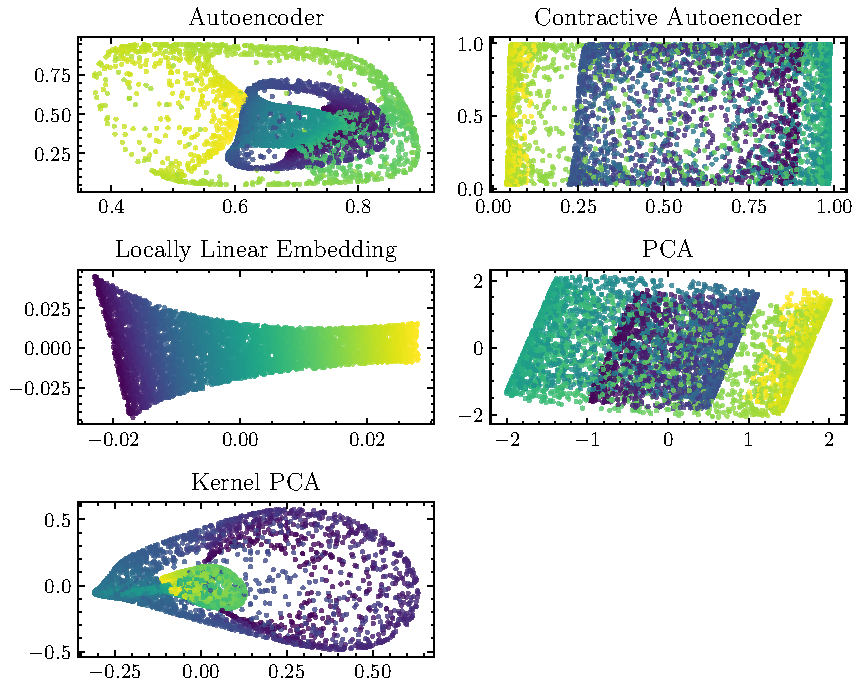
\includegraphics{SwissRollEmbeddings.pdf}
	\caption[Latente zweidimensionale Repräsentation $\mat{Y}$ fünf unterschiedlicher Methodes des Swiss Roll Datensatzes.]{Abgebildet sind die latenten zweidimensionalen Repräsentationen $\mat{Y}$ fünf unterschiedlicher Methoden des Swiss Roll Datensatzes. Nur Locally Linear Embedding ist in der Lage, die Swiss Roll zu \enquote{entfalten}. Dies ist angesichts der hohen Qualitätskriterien von Locally Linear Embedding und der niedrigeren Qualitätskriterien der restlichen Methoden auf diesem Datensatz stimmig (siehe \figref{fig:SwissRollMetrics}). (Eigene Darstellung)}
	\label{fig:SwissRollEmbeddings}
\end{figure}
die zweidimensionalen latenten Repräsentationen $\mat{Y} \in \real^{n \times 2}$ durch Anwendung der fünf Methoden auf den Swiss Roll Datensatz in einem Scatter-Plot dargestellt. Locally Linear Embedding ist als einzige Methode in der Lage, die Swiss Roll zu \enquote{entfalten}. Dies bestätigt die hohe Vertrauenswürdigkeit und Kontinuität der Dimensionsreduktion durch Locally Linear Embedding und die niedrigeren Werte der restlichen Methoden (siehe \figref{fig:SwissRollMetrics}). Die niedrigere Vertrauenswürdigkeit hat insbesondere für die Visualisierung eine große Bedeutung, da dies anzeigt, dass Punkte in der latenten Repräsentation Nachbarn werden, obwohl sie es ursprünglich nicht waren.

\subsection{Resultate auf natürlichen Datensätzen}
\label{ch:Vergleich:sec:Resultate:natuerlich}

Die Qualitätskriterien auf den natürlichen Datensätzen zeigen ein etwas anderes Bild, als es bei
den künstlichen Datensätzen der Fall war. Die starke Performance von Locally Linear Embedding setzt
sich nicht auf den natürlichen hochdimensionalen Datensätzen fort.
\begin{figure}[ht]
	\begin{center}
		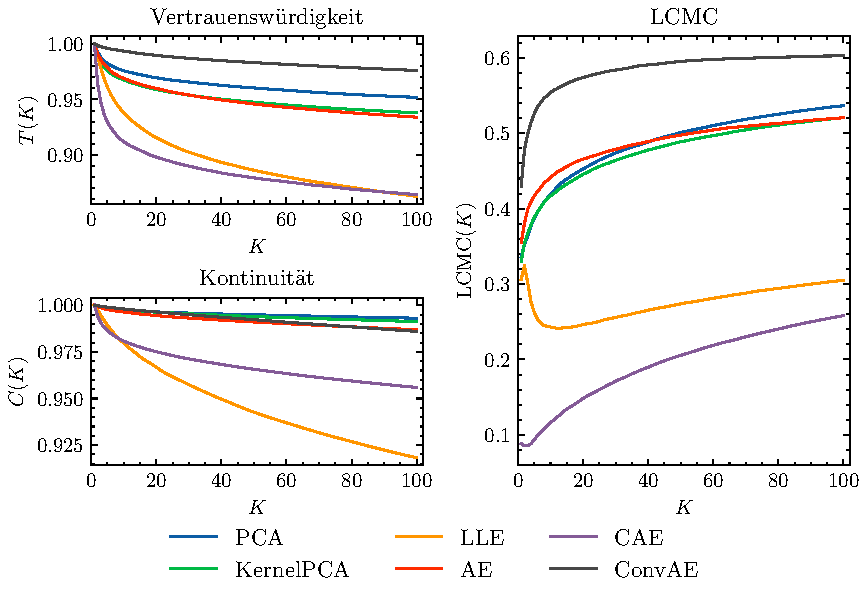
\includegraphics{MNIST_comparison.pdf}
	\end{center}
	\caption[Qualitätskriterien für MNIST]{Die Vertrauenswürdigkeit und Kontinuität der Dimensionsreduktion, sowie das Local Continuity Meta-Criterion (LCMC) für den MNIST-Datensatz. Auf diesem Datensatz kann der der domänenspezifische Convolutional Autoencoder (ConvAE) seine starke Performance zeigen, da der Datensatz von hoher Qualität ist und eine hohe Stichprobengröße aufweisen kann. Nichtsdestotrotz kann die Hauptkomponentenanalyse nur knapp dahinter gut mithalten und hinsichtlich der Kontinuität sogar übertreffen. Die Kernel PCA und der klassische vollvernetzte Autoencoder schneiden ebenfalls relativ gut ab, jedoch ist die Reduktion der Kernel PCA weniger vertrauenswürdig. Locally Linear Embedding und der Contractive Autoencoder können vor allem auf dem LCMC nicht mithalten. (Eigene Darstellung)}
	\label{fig:MNISTMetrics}
\end{figure}
Für die Olivetti Faces (\figref{fig:OlivettiFacesMetrics}), den FER- (\figref{fig:FER2013Metrics}) und den Fashion MNIST-Datensatz (\figref{fig:FashionMNISTMetrics})
schneidet LLE auf allen drei Kriterien relativ gesehen schlecht ab. insbesondere nehmen die
Qualitätskriterien von LLE mit größer werdender Nachbarschaftsgröße $K$ deutlicher ab, als bei den
restlichen Methoden. Aufgrund der Wahl der Nachbarschaftsgröße von $K=10$ für Locally Linear
Embedding und der lokalen Eigenschaften macht dies jedoch Sinn. Aus diesem Grund ist die
Betrachtung einer größeren Nachbarschaft der Qualitätskriterien für LLE benachteiligend, wurde aber
der Vollständigkeit halber und zu Vergleichszwecken trotzdem mit aufgenommen. Überraschenderweise
kann die Hauptkomponentenanalyse auf fast allen natürlichen Datensätzen eine gute oder sogar die
beste relative Performance aufweisen. Auf den vier Bilddatensätzen kann jedoch der Convolutional
Autoencoder seine Stärken zeigen, insbesondere wenn genügend Trainingsdaten zur Verfügung stehen. Letzteres trifft für MNIST-Datensatz \figref{fig:MNISTMetrics} zu, nicht jedoch für den Olivetti Faces-Datensatz.
Auf diesem Datensatz leidet die Performance der Autoencoder generell (siehe z.B. \figref{fig:OlivettiFacesMetrics}). Das Problem einer geringen Menge an Trainingsdaten gilt gleichermaßen für alle
Varianten von neuronalen Netzen, insbesondere jedoch für vollvernetzte Autoencoder aufgrund der
hohen Anzahl an Freiheitsgraden im Netz.

\subsubsection{Vergleich der Rekonstruktionen}

Interessant ist außerdem, wie gut die Dimensionsreduktionsmethoden ein originales Bild wieder
rekonstruieren können. In diesem Vergleich können allerdings nur die Hauptkomponentenanalyse und
alle Varianten der Autoencoder für die Rekonstruktion verwendet werden. Kernel PCA und Locally
Linear Embedding erlauben ohne Approximation keine inverse Transformation aus der latenten
Repräsentation $\vect{y}$ zurück in eine approximierte ursprüngliche Repräsentation
$\estNormal{\vect{x}}$. Für die Hauptkomponentenanalyse, den klassischen vollvernetzten
Autoencoder, den Convolutional Autoencoder und für den Contractive Autoencoder wurde auf dem
MNIST-Datensatz je ein Beispielbild für eine der Zahlen rekonstruiert und in
\figref{fig:MNIST-reconstructions} abgebildet. Die erste Zeile besteht aus den Originalbildern als
Referenz.
\begin{figure}[ht]
	\centering
	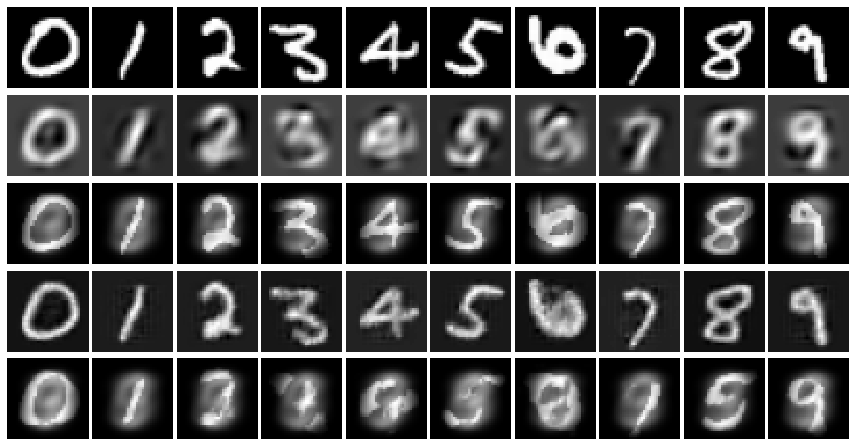
\includegraphics{reconstructions_mnist_pca_ae_convae_cae.pdf}
	\caption[Rekonstruierte MNIST-Zahlen]{Gezeigt sind einige rekonstruierten Zahlen aus dem MNIST-Datensatz von mehreren Methoden. Jede Zeile gehört zu einer Methode. Von oben nach unten: (1) Originale Bilder als Referenz, (2) Rekonstruktion durch PCA, (3) Rekonstruktion durch einen vollvernetzten Autoencoder, (4) Rekonstruktion durch den Convolutional Autoencoder und (5) Rekonstruktion durch den Contractive Autoencoder.}
	\label{fig:MNIST-reconstructions}
\end{figure}
Visuell ist die beste Rekonstruktion die des Convolutional Autoencoders, gefolgt vom vollvernetzten Autoencoder. Insbesondere die Rekonstruktionen des Contractive Autoencoders sind nicht gut, da einige Zahlen sogar als falsche Zahl rekonstruiert werden. Die Rekonstruktionen der Hauptkomponentenanalyse sind besser, aber visuell ebenfalls nicht überzeugend, da sie deutlich unscharfer sind. Der hier eingesetzte tiefe Convolutional Autoencoder mit mehr als 10 Schichten hat über zwölf Millionen trainierbare Gewichte und zeigt auf dem MNIST-Datensatz hinsichtlich der Qualitätskriterien eine gute Güte der Dimensionsreduktion (siehe \figref{fig:MNISTMetrics}). Allerdings ist MNIST ein relativ simpler Datensatz von hoher Qualität, so dass dieser tiefe Autoencoder scheinbar eine sinnvolle Repräsentation lernen kann. Beispielsweise ist der FER-Datensatz deutlich komplexer als MNIST mit einer geringeren Anzahl an Trainingsdaten. Auf diesen Datensätzen ist die Rekonstruktion des Convolutional Autoencoders nicht mehr so gut wie auf dem MNIST-Datensatz.

\subsubsection{Vergleich der Laufzeiten}

Nicht zu vernachlässigen ist der zeitliche Aufwand, den die Methoden auf den Datensätzen aufweisen.
Dazu sind in \tabref{tab:training_times} die Laufzeiten aller Methoden für alle Datensätze
aufgelistet.

\def\sym#1{\ifmmode^{#1}\else\(^{#1}\)\fi}
\begin{table}[ht]
	\centering
	\ra{1.3}
	\resizebox{\textwidth}{!}{
		\begin{tabular}{l*7{S[table-align-text-post=false]}}
			\toprule
			\multirow{2}[2]{*}{Methode} & \multicolumn{7}{c}{Laufzeit in Sekunden}                                                                                                                        \\
			\cmidrule{2-8}              & {MNIST}                                  & {Fashion MNIST}  & {Twin Peaks}    & {Swiss Roll}     & {ORL}           & {ICMR}          & {FER}                    \\
			\midrule
			PCA                         & 2,00                                     & 2,54             & 0,01            & 0,00             & 0,35            & 0,78            & 2,51                     \\
			Kernel PCA                  & 101,00\sym{*}                            & 101,72\sym{*}    & 0,62            & 0,59             & 0,03            & 1,01            & 103,17\sym{*}            \\
			LLE                         & 417,41\sym{**}                           & 447,95\sym{**}   & 0,45            & 0,42             & 0,24            & 1,14            & \bfseries 426,50\sym{**} \\
			AE                          & 161,35                                   & 121,14           & \bfseries 45,32 & \bfseries 102,34 & 43,02           & 54,51           & 102,26                   \\
			CAE                         & 403,74                                   & 641,00           & 30,04           & 22,68            & 5,76            & \bfseries 93,06 & 361,72                   \\
			ConvAE                      & \bfseries 467,61                         & \bfseries 754,83 & {--}            & {--}             & \bfseries 50,20 & {--}            & 249,64                   \\
			\bottomrule
			\multicolumn{8}{l}{\footnotesize Hinweis: Die Berechnung erfolgte auf einer zufällig gezogenen Teilmenge der Größe (\sym{*}) \num{15000} bzw. (\sym{**}) \num{20000}}                         \\
		\end{tabular}
	}
	\caption[Laufzeiten der Dimensionsreduktionsmethoden in Sekunden.]{Laufzeiten der einzelnen Dimensionsreduktionsmethoden in Sekunden (niedriger ist besser). Alle statistischen Methoden wurden auf einer Intel Xeon Gold 5315Y CPU mit \num{3,20} GHz Taktfrequenz und alle Machine Learning Methoden auf einer NVIDIA RTX A4000 Grafikkarte trainiert. Die höchsten Werte pro Datensatz wurden fett markiert. PCA weist auf allen Datensätzen, inklusive der etwas größeren Datensätze MNIST und Fashion MNIST, eine kurze Laufzeit von maximal \num{2,5} Sekunden auf. Die Laufzeiten der anderen beiden statistischen Methoden Kernel PCA und LLE steigen bei Datensätzen mit einer höheren Stichprobengröße stark an. Die längsten Laufzeiten weisen der Convolutional und Contractive Autoencoder auf.}
	\label{tab:training_times}
\end{table}

Die Hauptkomponentenanalyse weist die durschnittlich geringste Laufzeit auf und untermauert die bereits gute Perfomance auf den Qualitätskriterien. Die Laufzeiten von Locally Linear Embedding sind auf kleineren Datensätzen noch kurz, steigen aber mit der Stichprobengröße stark an. Die höchsten Laufzeiten weist der Convolutional Autoencoder auf dem MNIST-Datensatz mit 755 Sekunden oder circa 13 Minuten auf. Der Contractive Autoencoder hat ebenfalls auf den größeren Datensätzen eine hohe Laufzeit. Dies ist unter anderem der allgemeinen Implementierung des kontrahierenden Fehlerterms geschuldet. Eine spezifische Implementierung wie in \eqref{eq:CAE-loss-simple} könnte die Laufzeiten des Contractive Autoencoders noch verbessern, schränken dafür aber die Architektur in diesem Fall auf dreischichtige Autoencoder mit Sigmoid-Aktivierungsfunktionen ein.

\subsection{PCA und Autoencoder}
\label{ch:Vergleich:sec:Resultate:PCA_AE}

In diesem Abschnitt wird die Hauptkomponentenanalyse mit Autoencodern verglichen. Dazu wird zuerst
der theoretische Zusammenhang zwischen den beiden Methoden erklärt. Im Anschluss wird die
Hauptkomponentenanalyse und unterschiedliche Modelle des Autoencoders für einen empirischen
Vergleich auf dem FER-Datensatz trainiert, wobei aufgrund der sieben unterschiedlichen Emotionen im
Datensatz eine Reduktion auf sieben Dimensionen durchgeführt wurde. Ein Beispielbild für jede
Emotion des FER-Datensatzes ist in \figref{fig:FER-Datensatz-Beispiele} dargestellt.

\begin{figure}[ht]
	\centering
	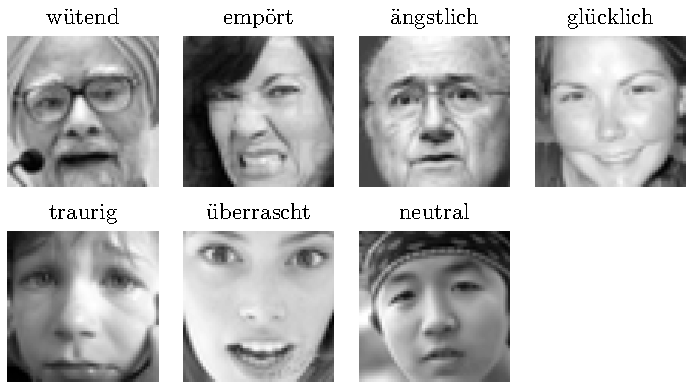
\includegraphics{fer2013-images.pdf}
	\caption[Beispielbilder des FER-Datensatzes]{Abgebildet ist je ein Bild für eine der sieben Emotionen im FER-Datensatz.}
	\label{fig:FER-Datensatz-Beispiele}
\end{figure}

\textcites{Baldi.1989}{Bourlard.1988} haben gezeigt, dass die Kodierung $\vect{y} = f(\vect{x})$ (siehe \secref{ch:MethodenDerDimRed:ML:AE:MathematischeFormulierung}) eines linearen Autoencoders äquivalent -- aber nicht identisch -- zu den Hauptkomponenten $\tr{\mat{A}}\vect{x}$ der PCA (siehe \secref{ch:MethodenDerDimRed:statistisch:PCA:HerleitungPC}) ist: Die Gewichte eines linearen Autoencoders, der den quadrierten Fehler (\eqref{eq:AE_objectiveFunction}) minimiert, spannen den gleichen Unterraum auf, wie die Ladungsmatrix $\mat{A}$. Dies gilt sogar dann, wenn im Encoder eines dreischichtigen Autoencoders Sigmoid-Aktivierungsfunktionen verwendet werden \parencite[291, 293]{Bourlard.1988}. Jedoch unterscheidet sich die latente Repräsentation $\mat{Y}$
eines linearen Autoencoders mit der von PCA wie folgt \parencite[3]{Plaut.2018}: (1) Die Kovarianzmatrix von $\mat{Y}$ ist nicht diagonal, das heißt die
latente Repräsentation ist nicht unkorreliert.\footnote{Äquivalent dazu ist die Korrelationsmatrix
	von $\mat{Y}$, welche lediglich eine skalierte Kovarianzmatrix darstellt, keine Einheitsmatrix.}
(2) Die transformierten Daten $\mat{Y}$ sind nicht nach absteigender Varianz sortiert. (3) Hat man
einen Encoder $f: \real^D \rightarrow \real^{k_1}$ und möchte man einen Vektor $\vect{x} \in
	\real^D$ auf nur $k_2$ Dimensionen mit $k_2 < k_1$ reduzieren, so können nicht einfach die ersten
$k_2$ Koordinaten von $f(\vect{x})$ verwendet werden. Das bedeutet, dass die Lösungen von
Autoencodern auf unterschiedliche Dimensionen nicht geschachtelt sind.

\begin{figure}[ht]
	\centering
	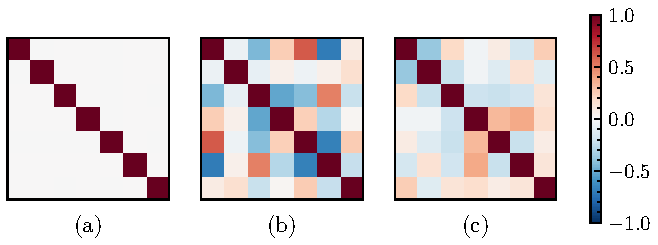
\includegraphics{correlation-matrices.pdf}
	\caption[Korrelationsmatrizen der transformierten Daten $\mat{Y}$ für den FER-Datensatz von vier Methoden]{Hier sind die Korrelationsmatrizen der transformierten Daten $\mat{Y}$ für den FER-Datensatz abgebildet, wobei in \captiona die Hauptkomponentenanalyse, in \captionb ein linearer dreischichtiger Autoencoder und in \captionc die linken Singulär-Vektoren der Decoder-Gewichtsmatrix eines linearen dreischichtigen Autoencoders, um die Daten auf sieben Dimensionen zu reduzieren. Die Korrelationsmatrix bei Transformation mittels der Hauptkomponentenanalyse ist per Konstruktion eine Einheitsmatrix, das heißt es besteht keine Korrelation in $\mat{Y}$. Bei Transformation durch den Autoencoder besteht Korrelation. Wendet man die Singulärwertszerlegung auf die Decoder-Gewichtsmatrix des linearen Autoencoders an, erhält man deutlich weniger Korrelation. Sie konnte aber nicht vollständig eliminiert werden. (Eigene Darstellung, angelehnt an \textcite[5]{Plaut.2018})}
	\label{fig:Korrelationsmatrizen}
\end{figure}
Punkt 1 ist beispielsweise in \figref{fig:Korrelationsmatrizen} zu erkennen. Dargestellt sind die Korrelationsmatrizen der transformierten Daten, wobei in \captiona die Hauptkomponentenanalyse, in \captionb ein linearer dreischichtiger Autoencoder und in \captionc ein nichtlinearer Autoencoder\rewrite{Hier erklären was man gemacht hat mit SVD} verwendet wurde. Die Korrelationsmatrix der Hauptkomponentenanalyse ist eine Einheitsmatrix, während die Korrelationsmatrizen der durch die Autoencoder gefundenen latenten Repräsentationen von Null verschiedene Werte auf der Nicht-diagonalen aufweisen.

Um die gefundenen Lösungen einer Hauptkomponentenanalyse und von Autoencodern genauer betrachten zu
können, kann die Ladungsmatrix $\mat{A}$ mit den Gewichtsmatrizen eines dreischichtigen
Autoencoders verglichen werden. Im Falle eines dreischichtigen Autoencoders sind die Gewichte des
Encoders eine Matrix $\mat{W}_1 \in \real^{d \times D}$ und die Gewichte des Decoders eine Matrix
$\mat{W}_2 \in \real^{D \times d}$. Auf Bilddatensätzen können diese Matrizen so umgeformt werden,
dass sich für jede Zeile von $\mat{W}_1$ oder Spalte von $\mat{W}_2$ ein Bild ergibt. Auf diese
Weise kann die \enquote{Arbeitsweise} des Autoencoders anschaulich untersucht werden.
\figref{fig:Gewichtsvergleich} setzt dieses Vorgehen auf dem FER-Datensatz um.
\begin{figure}[ht]
	\centering
	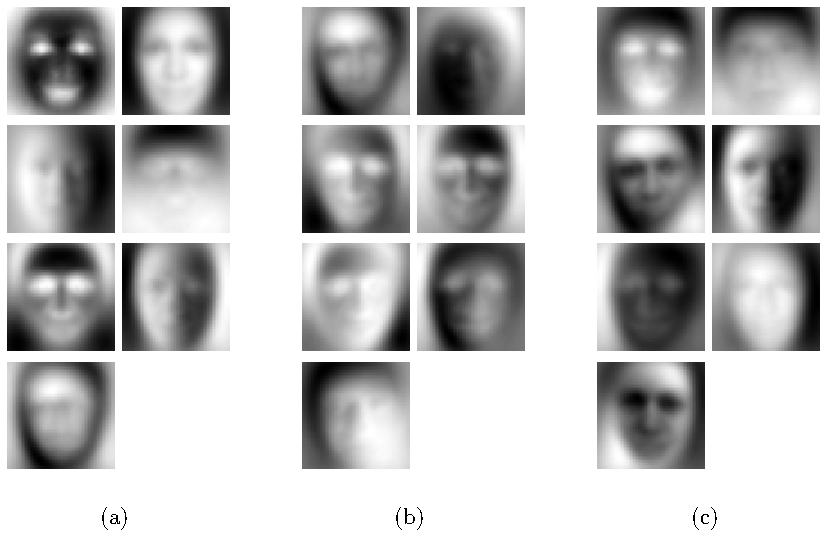
\includegraphics{weights-comparison.pdf}
	\caption[Die Gewichtsmatrizen von ausgewählten Methoden auf dem FER-Datensatz]{Gezeigt sind die Gewichtsmatrizen von drei Methoden bei einer Reduktion des FER-Datensatzes auf sieben Dimensionen. Ein einzelnes Bild entspricht einer Spalte der Ladungs- beziehungsweise Gewichtsmatrix, welche in die Größe des Bildes umgeformt wurde. \captiona Die Ladungsmatrix $\mat{A}$ der Hauptkomponentenanalyse, \captionb die Decoder-Gewichtsmatrix eines linearen dreischichtigen Autoencoders und \captionc die Decoder-Gewichtsmatrix eines nichtlinearen dreischichtigen Autoencoders, wobei der Encoder eine Sigmoid-Aktivierungsfunktion einsetzt und der Decoder linear ist. (Eigene Darstellung, angelehnt an \textcite[5]{Plaut.2018})}
	\label{fig:Gewichtsvergleich}
\end{figure}
Hierbei ist in \captiona die Ladungsmatrix von PCA, in \captionb die Gewichtsmatrix $\mat{W}_2$ eines linearen dreischichtigen Autoencoders und in \captionc die Gewichtsmatrix $\mat{W}_2$ eines nichtlinearen Autoencoders dargestellt. Wie zu erkennen ist, sind
die Gewichte des linearen Autoencoders bis auf das Vorzeichen sehr ähnlich zur Ladungsmatrix von
PCA.